\section{Topologies of Transformation Networks}
\label{chap:classification:topologies}

\mnote{Topology effects}
Due to our assumption of \emph{universality} (see \autoref{chap:introduction}), we have allowed arbitrary topologies of transformation networks in our approaches for achieving correctness of transformation networks.
The topology of a transformation network does, however, directly influence how prone it is to incorrectness and also to the fulfillment of other quality properties, which we have introduced in the previous section.
We consider the effects of a topology to different properties of transformation networks, for which we first discuss the extreme cases of topologies that have extreme effects on its properties.


\subsection{Topology Categories}

\mnote{Topology extremes}
Transformation networks induce a graph of metamodels as nodes and transformations as edges.
In general, this graph has an arbitrary topology, as there can be transformations between any pair of metamodels, and, in particular, there can be multiple paths of transformations between two metamodels in this graph.
As we have discussed in the previous section, properties of transformation networks are especially influenced by the presence of multiple paths of transformations between the same metamodels.
Thus, the density of the graph has gradual influence on the quality properties of the network.
Two extremes of topologies contain the minimum and maximum numbers of paths between each pair of metamodels.
They are given by complete graphs and trees, as exemplarily depicted in \autoref{fig:classification:topologies}.
While complete graphs contain an edge between each pair of nodes, i.e., one transformation between each pair of metamodels, a tree contains only one path between each pair of nodes, i.e., only one sequence of transformations between two metamodels.
We have already discussed the effects of these extremes in previous work~\owncite{klare2018docsym}.

\begin{figure}
    \centering
    \begin{minipage}[b]{0.49\columnwidth}
        \centering
        \newcommand{\hmmdistance}{3.6em}
\newcommand{\vmmdistance}{2.4em}

\begin{tikzpicture}[
    mm/.style={schematic metamodel},
]

\node[mm] (full_left) {};
\node[mm, above right=\vmmdistance and \hmmdistance of full_left.center, anchor=center] (full_top) {};
\node[mm, below right=\vmmdistance and \hmmdistance of full_left.center, anchor=center] (full_bottom) {};
\node[mm, right=2*\hmmdistance of full_left.center, anchor=center] (full_right) {};
\node[mm, below left=\vmmdistance and \hmmdistance of full_left.center, anchor=center] (full_bottomleft) {};

\draw[transformation] (full_left) -- (full_top);
\draw[transformation] (full_left) -- (full_right);
\draw[transformation] (full_left) -- (full_bottom);
\draw[transformation] (full_top) -- (full_right);
\draw[transformation] (full_top) -- (full_bottom);
\draw[transformation] (full_right) -- (full_bottom);
\draw[transformation] (full_left) -- (full_bottomleft);
\draw[transformation] (full_bottom) -- (full_bottomleft);
\draw[transformation] (full_top) to[bend right=30] (full_bottomleft);
\draw[transformation] (full_bottomleft) .. controls ++(1*\hmmdistance, -0.8*\vmmdistance) and ([yshift=-1.5*\vmmdistance]full_right.south) .. (full_right);

\end{tikzpicture}
        \subcaption{Complete graph}
        \label{fig:classification:topologies:complete}
    \end{minipage}
    \hfill
    \begin{minipage}[b]{0.49\columnwidth}
        \centering
        \newcommand{\hmmdistance}{3.6em}
\newcommand{\vmmdistance}{2.4em}

\begin{tikzpicture}[
    mm/.style={schematic metamodel}
]

\node[mm, right=4*\hmmdistance of full_left.center, anchor=center] (tree_left) {};
\node[mm, above right=\vmmdistance and \hmmdistance of tree_left.center, anchor=center] (tree_top) {};
\node[mm, below right=\vmmdistance and \hmmdistance of tree_left.center, anchor=center] (tree_bottom) {};
\node[mm, right=2*\hmmdistance of tree_left.center, anchor=center] (tree_right) {};
\node[mm, below left=\vmmdistance and \hmmdistance of tree_left.center, anchor=center] (tree_bottomleft) {};

\draw[transformation] (tree_left) -- (tree_top);
\draw[transformation] (tree_left) -- (tree_bottom);
\draw[transformation] (tree_left) -- (tree_bottomleft);
\draw[transformation] (tree_top) -- (tree_right);

\end{tikzpicture}
        \vspace{1em}
        \subcaption{Tree}
        \label{fig:classification:topologies:tree}
    \end{minipage}
    \caption[Extremes of transformation network topologies]{Examples for extreme topologies of transformation networks with five metamodels. Nodes depict metamodels and edges depict transformations. Adapted from~\owncite[Fig.~2]{klare2018docsym}.}
    \label{fig:classification:topologies}
\end{figure}

\mnote{Complete graphs}
In a complete graph (see \autoref{fig:classification:topologies:complete}), each node is connected to each other by an edge.
In consequence, each of the $n$ nodes has $n-1$ edges to the other nodes, leading to a total of $\frac{n*(n-1)}{2}$ edges.
This conforms to the number of transformations defined in a transformation network that induces a complete graph.
In addition, the paths of transformations between two metamodels are given by paths of all lengths between $1$ and $n-2$ involving all permutations of the remaining $n-2$ metamodels.
This leads to $\sum_{i=0}^{n-2} \frac{(n-2)!}{(n-2-i)!} = \sum_{i=0}^{n-2} \binom{n-2}{i} i!$ transformation paths between each pair of metamodels.

\mnote{Dense graphs in practice}
In practice, the induced graph of a transformation network will, of course, usually not be complete but a graph of arbitrary density, in which there may be clusters of complete subgraphs.
Imagine the development of an automobile, in which models from different domains, such as electrical engineering, mechanical engineering, and software engineering, are involved. 
While models within one domain may all be related by transformations, there may be specific interface models that are used to relate the models of one domain to those of the others, which avoids the necessity to have knowledge about the relations between all models across existing domain borders.

\mnote{Trees}
In a tree (see \autoref{fig:classification:topologies:tree}), there is only one path between each pair of nodes.
Thus, a tree of $n$ nodes has $n-1$ edges.
A transformation network that induces a tree thus has a number of transformations reduced by a factor of $\frac{n}{2}$ in comparison to a complete graph and an even greater reduction in the number of transformation paths between two metamodels.
This leads to significant advantages regarding interoperability of the transformations, which we categorize in more detail in the following.

\mnote{Natural topologies}
A transformation network inducing a complete graph can naturally be achieved by expressing each consistency relation in a transformation.
If two metamodels are not related at all, the according transformation does nothing.
Defining a tree is, however, more complex, as it imposes severe restriction regarding the transformations in which relations have to be preserved to avoid having two paths of transformations between the same metamodels.
In the following, we discuss the effects of these extreme topologies and derive which inherent property guarantees a specific topology can give.


\subsection{Effects on Properties}
\label{chap:classification:topologies:effects}

\mnote{Extreme property effects}
We have discussed in \autoref{chap:classification:properties} how the existence of multiple transformation paths between two metamodels affects quality properties of transformation networks.
In the previous subsection, we have identified complete graphs and trees as two extremes of topologies of transformation networks that have particular effects on the existence of such multiple paths.
These topology extremes have extreme effects on the quality properties of a network.

\begin{propertable}
    \renewcommand{\arraystretch}{1.2}
    \newcommand{\cc}{\cellcolor{\secondlinecolor}}
    \begin{tabular} {L{7.5em} L{6.5em} C{7.5em} C{7em}}
        \toprule
        \textbf{Category} & \textbf{Property} & \textbf{Complete Graph} & \textbf{Tree} \\
        \midrule
        \multirow{2}{*}{Functionality} &
        \cc Correctness & \cc - & \cc ++ \\
        & Completeness & ++ & - \\
        \midrule
        \multirow{5}{*}{Maintainability} &
        \cc Modularity & \cc - & \cc + \\
        & Reusability & ++ & - \\
        & \cc Analyzability & \cc - & \cc + \\
        & Modifiability & - & + \\
        & \cc Testability & \cc - & \cc + \\
        \bottomrule
    \end{tabular}
    \caption[Topology effects on quality properties]{Effects of topology extremes on quality properties. \enquote{+} and \enquote{-} indicate whether a topology improves or degrades a property, \enquote{++} denotes inherent optimization of the property.}
    \label{tab:classification:topology_impact}
\end{propertable}

\mnote{Summary of topology effects of properties}
\autoref{tab:classification:topology_impact} summarizes the impact of topologies on quality properties.
The classification is only based on the existence of multiple transformation paths between the same pairs of metamodels, as we have discussed in \autoref{chap:classification:properties}.
There are, of course, more influencing factors that can improve or degrade these properties.
In fact, we are particularly interested in properties that are inherently optimized by specific topologies, which are functional correctness and completeness as well as reusability.

\mnote{Slight maintainability effects}
Modularity, analyzability, modifiability, and testability all benefit from the absence of multiple transformation paths between the same metamodels, because the information about one relation is only located at one place, which can be a single transformation or a single sequence of them.
But the information is not duplicated across several transformation paths.
Since we expect a benefit from the absence of duplications for the mentioned properties, we classify them as improved by tree topologies and degraded by complete graphs.
There are, however, further influencing factors that may mitigate this classification.
For example, to achieve a tree it is necessary to express at least some of the relations indirectly across multiple transformations, as not each relation can be expressed directly.
This can degrade properties like modifiability, as it gets more complicated to comprehend relations if they are defined across multiple transformations rather than in a single one.

\begin{figure}
    \centering
    \newcommand{\mmdistance}{4em}

\begin{tikzpicture}[
    mm/.style={schematic metamodel},
]

% graph

\node[mm] (graph_top) {};
\node[mm, below=\mmdistance of graph_top.center, anchor=center] (graph_middle) {};
\node[mm, below left=0.5*\mmdistance and sqrt(3)/2*\mmdistance of graph_middle.center, anchor=center] (graph_bottomleft) {};
\node[mm, below right=0.5*\mmdistance and sqrt(3)/2*\mmdistance of graph_middle.center, anchor=center] (graph_bottomright) {};

\draw[consistency relation] (graph_top) -- node[left] {$\consistencyrelation{CR}{2}$} (graph_middle);
\draw[consistency relation] (graph_top) to[bend right=40] node[pos=0.3, above left] {$\consistencyrelation{CR}{1}$} (graph_bottomleft);
\draw[consistency relation] (graph_top) to[bend left=40] node[pos=0.3, above right] {$\consistencyrelation{CR}{3}$} (graph_bottomright);
\draw[consistency relation] (graph_middle) -- node[pos=0.4, above left] {$\consistencyrelation{CR}{4}$} (graph_bottomleft);
\draw[consistency relation] (graph_middle) -- node[pos=0.4, above right] {$\consistencyrelation{CR}{5}$} (graph_bottomright);

% tree

\node[mm, right=4.5*\mmdistance of graph_top] (tree_top) {};
\node[mm, below=\mmdistance of tree_top.center, anchor=center] (tree_middle) {};
\node[mm, below left=0.5*\mmdistance and sqrt(3)/2*\mmdistance of tree_middle.center, anchor=center] (tree_bottomleft) {};
\node[mm, below right=0.5*\mmdistance and sqrt(3)/2*\mmdistance of tree_middle.center, anchor=center] (tree_bottomright) {};

\draw[consistency relation] (tree_top) -- node[left] {$\consistencyrelation{CR}{2}$} (tree_middle);
\draw[consistency relation] (tree_middle) -- node[pos=0.4, above left] {$\consistencyrelation{CR}{4}$} (tree_bottomleft);
\draw[consistency relation] (tree_middle) -- node[pos=0.4, above right] {$\consistencyrelation{CR}{5}$} (tree_bottomright);


\draw[latex-latex] ([yshift=0.2*\mmdistance, xshift=1.1*\mmdistance]graph_middle.east) -- 
    node[above] {$\consistencyrelation{CR}{2} \concat \consistencyrelation{CR}{4} \subseteq \consistencyrelation{CR}{1}$} 
    node[below] {$\consistencyrelation{CR}{2} \concat \consistencyrelation{CR}{5} \subseteq \consistencyrelation{CR}{3}$}
    ([yshift=0.2*\mmdistance, xshift=-1*\mmdistance]tree_middle.west);

\end{tikzpicture}
    \caption[Equality of graph and tree of consistency relations]{Example for consistency relations in a graph that can be equally represented by consistency relations in a tree. Adapted from~\owncite[Fig.~3]{klare2018docsym}.}
    \label{fig:classification:tree_generation}
\end{figure}

\mnote{Completeness in complete graphs}
Completeness and reusability are inherently given in networks inducing a complete graph.
A complete graph of transformations allows to preserve consistency to any set of binary consistency relations, as the topology does not restrict between which metamodels transformations are allowed to be expressed.
Trees, on the other hand, do not allow to express every set of relations, as we have already motivated in \autoref{chap:introduction:challenges:quality:properties}.
If, for example, the \gls{PCM}, the \gls{UML}, and Java all share information pairwise, which cannot be expressed in instances of the third metamodel, there is no tree of transformations that preserves consistency for all this information.
In general, of three metamodels there must always be one that is able to express the information shared between the other two to encode their consistency preservation in a tree of transformations.
Transferred to \modellevelconsistencyrelations (see \autoref{def:modellevelconsistencyrelation}), this means that between three metamodels there must be a concatenation of two consistency relations that is a subset of the third.
In that case, the third relation is subsumed by the concatenation of the others anyway and can thus be omitted.
This situation is depicted in \autoref{fig:classification:tree_generation}.

\mnote{Reusability in complete graphs}
In addition, reusability is given by complete graphs, because preserving consistency between two metamodels is always represented in a direct transformation between them, which can readily be reused.
From a transformation network inducing a tree, only subtrees of transformations can be reused without loosing guarantees for consistency preservation.
If, for example, \gls{PCM} and Java models are kept consistent via the \gls{UML}, it is not possible to reuse the (indirectly expressed) transformation between Java and \gls{PCM} without reusing the \gls{UML}.
This significantly restricts reusability in tree topologies.

\mnote{Correctness in trees}
Correctness, on the other hand, is inherently given in networks inducing a tree topology.
Between each pair of metamodel there is only one path of transformations.
In consequence, there cannot be any incompatibility (see \autoref{chap:compatibility}), as this requires multiple contradicting sequences of consistency relations encoded into transformations.
In addition, transformations do not need to be synchronizing (see \autoref{chap:synchronization}), as the situation that both models involved in a transformation have been modified is never given due to the missing situation of multiple transformation paths modifying the same models.
Finally, only the orchestration of transformations (see \autoref{chap:orchestration}) remains a challenge in such trees.
Although there are no cycles of transformations that need to be orchestrated, and thus any topological order of transformations starting with the node representing the metamodel of the changed model may be selected, we have identified in \autoref{chap:orchestration} that it can be necessary to execute transformations multiple times, as they need to react to the changes performed by other transformations.
This already occurs when two transformations are chained.
Since this challenge does always occur when a transformation is able to change both involved models rather than only one of them, the only solution is to enforce transformations to only change one model, which may prevent relevant scenarios, as discussed in \autoref{chap:orchestration}.
The evaluation of our approaches for achieving correctness in \autoref{chap:correctness_evaluation}, however, indicates that issues due to orchestration of transformations may not be that relevant in practice.
Summarizing, apart from the discussed restrictions, this leads to inherent functional correctness as defined in \autoref{chap:correctness}.
Thus, in a network that induces a tree, several severe challenges for correctness of transformation networks do not occur.

% \begin{figure}
%     \centering
%     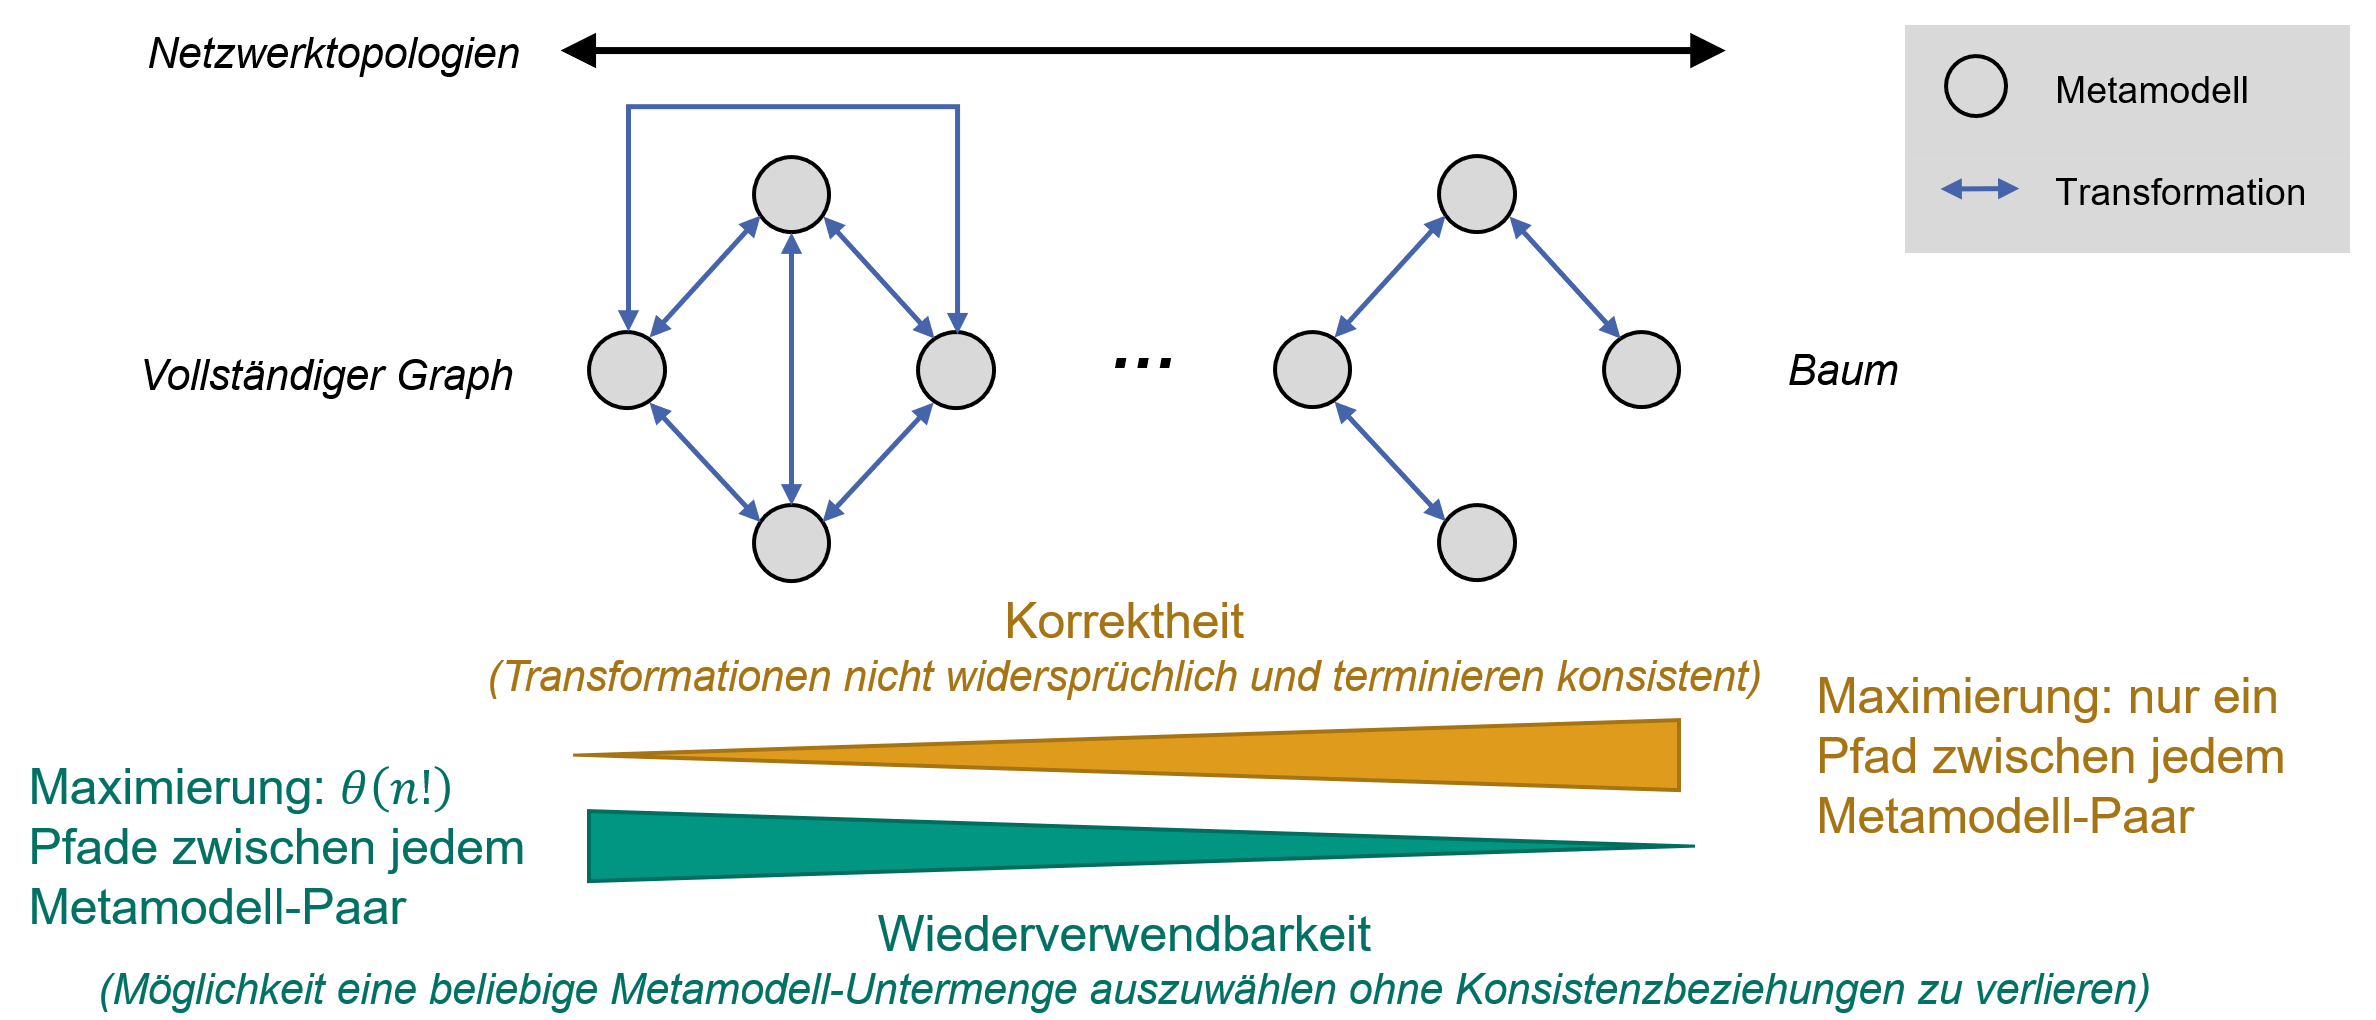
\includegraphics[width=\textwidth]{figures/quality/classification/tradeoff.png}
%     \caption[Trade-off between correctness and reusability]{Trade-off between quality properties at the example of correctness and reusability depending on the network topology.}
%     \label{fig:classification:tradeoff}
% \end{figure}

\mnote{Gradual improvement in actual networks}
An actual transformation network will usually neither induce a complete graph nor a tree, although we have already discussed that complete graphs are at least easier to achieve.
Thus, a network will not inherently optimize any of these properties but gradually optimize some of them, depending on the number of duplications of preservation for consistency relations within the transformations.
This leads to a trade-off between different properties depending on the achieved topology.
More duplications lead to higher completeness and reusability, whereas less duplications improve inherent correctness and also likely improve further discussed quality properties.

\mnote{Benefit of trees}
Although trees are not easy to achieve in practice due to the missing ability of transformation networks with such a topology to express all possible consistency relations, their inherent correctness guarantee is still interesting, as we have seen how difficult correctness is to achieve in networks of arbitrary topology in the previous chapters.
In the following chapter, we thus identify and discuss how we can use this essential benefit of trees to construct networks that still provide a high level of completeness and reusability.

\mnote{Fine-grained topology notion}
In fact, we have up to now discussed the topology of transformation networks at the level of complete metamodels and transformations between them.
Transformations are, however, composed of rules that preserve consistency according to fine-grained consistency relations, such as the ones we have specified in \autoref{def:consistencyrelation}.
Thus, we can even generalize the insights regarding topologies from complete metamodels and transformations to metamodel elements and fine-grained consistency relations, which then mitigates some of the drawbacks regarding completeness of trees.
This conforms to the notion of \emph{non-interference} defined by \textcite{stevens2020BidirectionalTransformationLarge-SoSym}, which considers transformations to be non-interfering as long as they affect independent subsets of the metamodels and then can be executed in any order.

